%!TEX root = ../main.tex

\section{chainerの基礎}
本章では,deeplearningのフレームワークの一つであるchainerについて基本的なコードを用いて説明する.
\subsection{開発環境について}
\subsubsection{sshについて}
配布したuser名,パスワードで以下のコマンドで開発環境にログインできる.

\begin{lstlisting}[basicstyle=\ttfamily\footnotesize, frame=single]
ssh Username@IPaddress
\end{lstlisting}
yes/noを聞かれるので,yesと入力した後,配られたパスワードを入力することでログインできる.

この工程を簡略化したい場合は,\url{https://qiita.com/ir-yk/items/af8550fea92b5c5f7fca},
\url{https://qiita.com/passol78/items/2ad123e39efeb1a5286b}などを参考にすること.
\subsubsection{scpについて}
コードを編集する際,リモートではなく,ローカルで編集しその結果をリモートに反映させたいという需要があると思う.
その際は,scpコマンドを用いる.
\begin{lstlisting}[basicstyle=\ttfamily\footnotesize, frame=single]
scp LocalFilePath Username@IP:RemotePath
\end{lstlisting}
と打てば,ローカル→リモートにファイルの転送ができる.その他の使い方については,\url{https://qiita.com/katsukii/items/225cd3de6d3d06a9abcb}などを参考にすること.

また,エディタによってはこういった機能をサポートしてくれるものもある.""使っているエディタ sftp""などで検索すると良い.

\subsubsection{tmuxについて}
開発環境でコードを実行していてもそのままだと,パソコンを閉じる,開発環境と接続を切るなどすると実行が終了してしまう.それを防ぐのがtmuxである.tmux上で実行すればこういった問題を解決できる.詳細については,
\url{https://qiita.com/vintersnow/items/be4b29652ff665c45198}などを参考にすること.
\subsection{サンプルコードの実行}
今回扱うサンプルコードはmnistと呼ばれる手書き数字の分類を行うものである.
\begin{practice}
train\_mnist\_mlp.pyをGPUで実行せよ.

次のコマンドを打つと学習を開始できる.
\begin{lstlisting}[basicstyle=\ttfamily\footnotesize, frame=single]
python train_mnist_mlp.py -g 0
\end{lstlisting}

\end{practice}
数分待つと,学習が終了し,resultフォルダに結果が出力されている.
\begin{figure}[ht]
	\begin{center}
		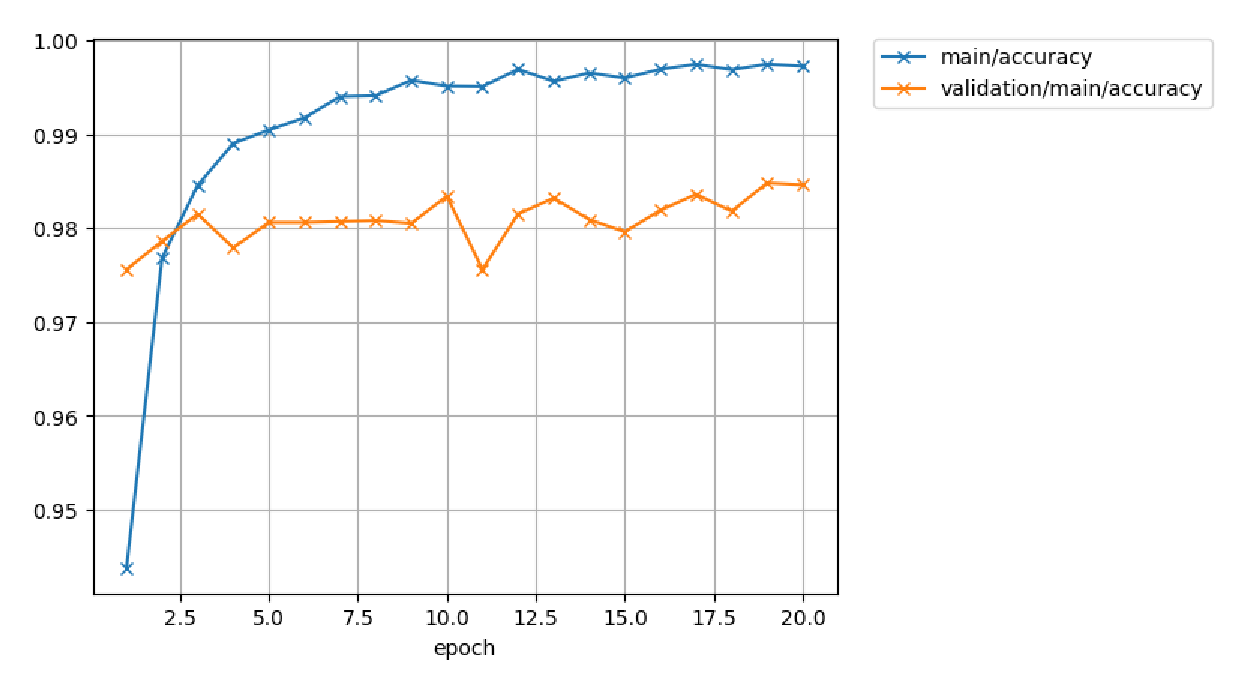
\includegraphics[width=0.7\linewidth] {images/YamasakiLab/sec2/accuracy.eps}
		\caption{学習結果の例}
		\label{fig:accuracy}
	\end{center}
\end{figure}


次に,学習がうまくできたか確認する.
\begin{practice}
白黒の手書き数字画像を作成せよ.
この時黒地に白文字で数字を書くことに注意する.(学習させた手書き数字データが黒地に白なので)
\end{practice}

\begin{figure}[ht]
	\begin{center}
		
\includegraphics[width=0.2\linewidth] {images/YamasakiLab/sec2/number.eps}
		\caption{手書き数字の例}
		\label{fig:num}
	\end{center}
\end{figure}

\begin{practice}
自分が書いた手書き文字を先程学習したモデルに通して出力を表示し,正しく数字が認識されたか確かめよ.
次のコマンドでテストコードを実行できる.
\begin{lstlisting}[basicstyle=\ttfamily\footnotesize, frame=single]
python test_mnist_mlp.py -g 0 -i (path to the input image) -m result/model_20
\end{lstlisting}

\end{practice}

\subsection{サンプルコードの解説}
先の章で実行したサンプルコードについて簡単に解説を行う.
chainerの公式ドキュメント(https://docs.chainer.org/en/stable/)を適宜参考にすること.

\subsubsection{コマンドライン引数}
% \pythonexternal{YamasakiLab/code/sec2_command.py}
\begin{lstlisting}[basicstyle=\ttfamily\footnotesize, frame=single]
    parser = argparse.ArgumentParser(description=‘Chainer example: MNIST’)
    parser.add_argument(‘--batchsize’, ‘-b’, type=int, default=100,
                        help=‘Number of images in each mini-batch’)
    parser.add_argument(‘--epoch’, ‘-e’, type=int, default=20,
                        help=‘Number of sweeps over the dataset to train’)
    parser.add_argument(‘--frequency’, ‘-f’, type=int, default=-1,
                        help=‘Frequency of taking a snapshot’)
    parser.add_argument(‘--gpu’, ‘-g’, type=int, default=-1,
                        help=‘GPU ID (negative value indicates CPU)‘)
    parser.add_argument(‘--out’, ‘-o’, default=‘result’,
                        help=‘Directory to output the result’)
    parser.add_argument(‘--resume’, ‘-r’, default=‘’,
                        help=‘Resume the training from snapshot’)
    parser.add_argument(‘--unit’, ‘-u’, type=int, default=1000,
                        help=‘Number of units’)
    args = parser.parse_args()
\end{lstlisting}
このプログラムで使うことのできるコマンドライン引数を定義している.各変数に対する説明は省略する.

\subsubsection{モデル}
% \pythonexternal{YamasakiLab/code/sec2_mlp.py}
\begin{lstlisting}[basicstyle=\ttfamily\footnotesize, frame=single]
 model = MLP(args.unit, 10)
     if args.gpu >= 0:
        # Make a specified GPU current
        chainer.cuda.get_device_from_id(args.gpu).use()
        model.to_gpu()  # Copy the model to the GPU
\end{lstlisting}
この行で今回の学習に用いるモデルを定義している.また,GPUを使用していたらモデルをGPUに変更していいる.args.gpuは使用するGPUの番号を示している.
MLP自体は以下で定義している.
\begin{lstlisting}[basicstyle=\ttfamily\footnotesize, frame=single]
class MLP(chainer.Chain):
    def __init__(self, n_units, n_out):
        super(MLP, self).__init__()
        with self.init_scope():
            self.l1 = L.Linear(None, n_units)  # n_in -> n_units
            self.l2 = L.Linear(None, n_units)  # n_units -> n_units
            self.l3 = L.Linear(None, n_out)  # n_units -> n_out

    def __call__(self, x, t=None):
        h = F.relu(self.l1(x))
        h = F.relu(self.l2(h))
        h = self.l3(h)

        loss = F.softmax_cross_entropy(h, t)
        accuracy = F.accuracy(h, t)
        chainer.report({‘loss’: loss}, self)
        chainer.report({‘accuracy’: accuracy}, self)

        if chainer.config.train:
            return loss
        else:
            return h

    def predict(self, x):
        h = F.relu(self.l1(x))
        h = F.relu(self.l2(h))
        h = self.l3(h)
        return h
\end{lstlisting}

init関数で今回使うネットワークの構造を定義しており,今回は入力層(l1),中間層(l2),出力層(l3)の全3層である.今回用いた層は全て全結合層である.
xがネットワークのinput,hがネットワークのoutput,tがinputの正解ラベルである.trainの時はlossを返し学習をさせており,validationの時は学習をさせたくないのでhを返している.(validationの時も学習させてしまうとvalidationのaccuracyが正当な評価にならない.)

\subsubsection{optimizer}
\begin{lstlisting}[basicstyle=\ttfamily\footnotesize, frame=single]
    # Setup an optimizer
    optimizer = chainer.optimizers.Adam()
    optimizer.setup(model)
\end{lstlisting}
この部分では,lossを最適化するための手法を決めておりこのプログラムではAdamを用いている.
他の最適化手法を用いたい場合はhttps://docs.chainer.org/en/stable/reference/optimizers.htmlなどを参考にすること.

\subsubsection{データセット}
\begin{lstlisting}[basicstyle=\ttfamily\footnotesize, frame=single]
   # Load the MNIST dataset
    train, test = chainer.datasets.get_mnist()
\end{lstlisting}
この部分では,今回の学習に用いるデータセットを定義している.今回用いたmnistのデータセットはchainerが用意してくれているのでこのように1行書くだけで呼び出せる.自分で用意したデータセットを用いたい場合については後の演習に譲る.
 
 \subsubsection{Trainerの準備}
\begin{lstlisting}[basicstyle=\ttfamily\footnotesize, frame=single]
    train_iter = chainer.iterators.SerialIterator(train, args.batchsize)
    test_iter = chainer.iterators.SerialIterator(test, args.batchsize,
                                                 repeat=False, shuffle=False)

    # Set up a trainer
    updater = training.StandardUpdater(train_iter, optimizer, device=args.gpu)
    trainer = training.Trainer(updater, (args.epoch, ‘epoch’), out=args.out)
\end{lstlisting}
 これまでに定義したものを用いて学習のためのTrainerを作成している.
  \subsubsection{modelの評価と結果の可視化}
\begin{lstlisting}[basicstyle=\ttfamily\footnotesize, frame=single]
    # Evaluate the model with the test dataset for each epoch
    trainer.extend(extensions.Evaluator(test_iter, model, device=args.gpu))

    trainer.extend(extensions.dump_graph(‘main/loss’))

    frequency = args.epoch if args.frequency == -1 else max(1, args.frequency)
    trainer.extend(extensions.snapshot(), trigger=(frequency, ‘epoch’))
    trainer.extend(extensions.snapshot_object(model, ‘model_{.updater.epoch}’),
                   trigger=(frequency, ‘epoch’))


    trainer.extend(extensions.LogReport())
    if extensions.PlotReport.available():
        trainer.extend(
            extensions.PlotReport([‘main/loss’, ‘validation/main/loss’],
                                  ‘epoch’, file_name=‘loss.png’))
        trainer.extend(
            extensions.PlotReport(
                [‘main/accuracy’, ‘validation/main/accuracy’],
                ‘epoch’, file_name=‘accuracy.png’))

    trainer.extend(extensions.PrintReport(
        [‘epoch’, ‘main/loss’, ‘validation/main/loss’,
         ‘main/accuracy’, ‘validation/main/accuracy’, ‘elapsed_time’]))

    trainer.extend(extensions.ProgressBar())
\end{lstlisting}
ここでは,学習結果の出力と可視化を主に行なっている.extensions.snapshot\_object関数は,学習したモデルを出力する関数で,triggerはその出力を何epoch毎に行うかを決定している.他の関数については説明を省略する.

ここまでが,train\_mnist\_mlp.pyの大まかな解説である.次にtest\_mnist\_mlp.pyの解説を行う.

 \subsubsection{訓練モデルの読み込み}
\begin{lstlisting}[basicstyle=\ttfamily\footnotesize, frame=single]
    model = MLP(args.unit,10)
    serializers.load_npz(args.model, model)
\end{lstlisting}
先ほど学習したモデルを読み込んでいる.先に学習したモデルと同じ形のモデルを作っておかないと読み込めないことに注意する.
 \subsubsection{画像の読み込み}
\begin{lstlisting}[basicstyle=\ttfamily\footnotesize, frame=single]
    try:
        img = Image.open(args.image).convert(“L”).resize((28,28))
    except :
        print(“invalid input”)
        return
\end{lstlisting}
画像を読み込み,mnistと同じサイズ(白黒,28*28)に変換している.

\subsubsection{結果の出力}
\begin{lstlisting}[basicstyle=\ttfamily\footnotesize, frame=single]
    img_array = np.asarray(img,dtype=np.float32).reshape(1,784)
    result = model.predict(img_array)
    print(“predict:“, np.argmax(result.data))
\end{lstlisting}
今回使用したネットワークは画像を2次元の形で入力するのではなく,1次元に潰して入力するので28*28を1*784にreshapeを行っている.モデルの出力は,[入力数字が0である確信度,入力数字が1である確信度,入力数字が2である確信度,...]となっているのでその配列のargmaxを取ることで最も確信度が高い数字つまり予測数字を出力している.model.predictの返り値がVariable型と呼ばれるものになっているので,
.dataを使うことで中身の配列にアクセスすることができる.
\begin{practice}
test\_mnist\_mlp.pyを書き換えることで予測数字を確信度が高い方から上位3つまで出すように変更せよ.
\end{practice}

\subsection{ネットワークの変更}

先の章で用いたネットワークは,中間層のノード数を変化させることができ,それによりモデルの精度,実行時間などが変化する.
\begin{practice}
MLPの中間ノード数を
\begin{enumerate}
\item 3
\item 10000
\end{enumerate}
にしてそれぞれ20epoch学習し,最終的な精度と学習にかかった時間を比較せよ.
\end{practice}

MLPはネットワークに画像を入力する際,2次元の画像を1次元に潰して入力してしまっている.それにより,隣接するピクセルの関係を用いた学習が難しくなってしまっている.そのため本来全結合のみのネットワークは画像の学習に適さない.そこで全結合層ではなく,畳み込み層を用いたネットワークで学習させることを考える.

\begin{practice}
net.pyを書き換えることで,下の図~\ref{fig:prac_cnn}のネットワークをMNIST\_CNNクラスに実装せよ.ただし,カーネルサイズはどちらの畳み込み層についても\(\left(5 \times 5 \right)\)とする.
MNIST\_CNNクラスを実装したら,train\_mnist\_cnn.pyを同様に実行することで精度を確かめよ.興味がある人は,test\_mnist\_mlp.pyを参考にテスト用のコードを書き実行せよ.
\begin{figure}[ht]
	\begin{center}
		\includegraphics[width=0.8\linewidth] {images/YamasakiLab/sec2/practice_cnn.eps}
		\caption{作成するCNN}
		\label{fig:prac_cnn}
	\end{center}
\end{figure}

ヒント : chainerのドキュメントでConvolution2Dを検索せよ.
\end{practice}

\subsection{他のデータセットでの学習}
先章では,mnistを題材として学習を行なったが,本章ではもう少し複雑なデータセットであるCIFAR-10を扱う.
CIFAR-10は10クラス,32*32のカラー画像のデータセットである.
\begin{figure}[h]
	\begin{center}
		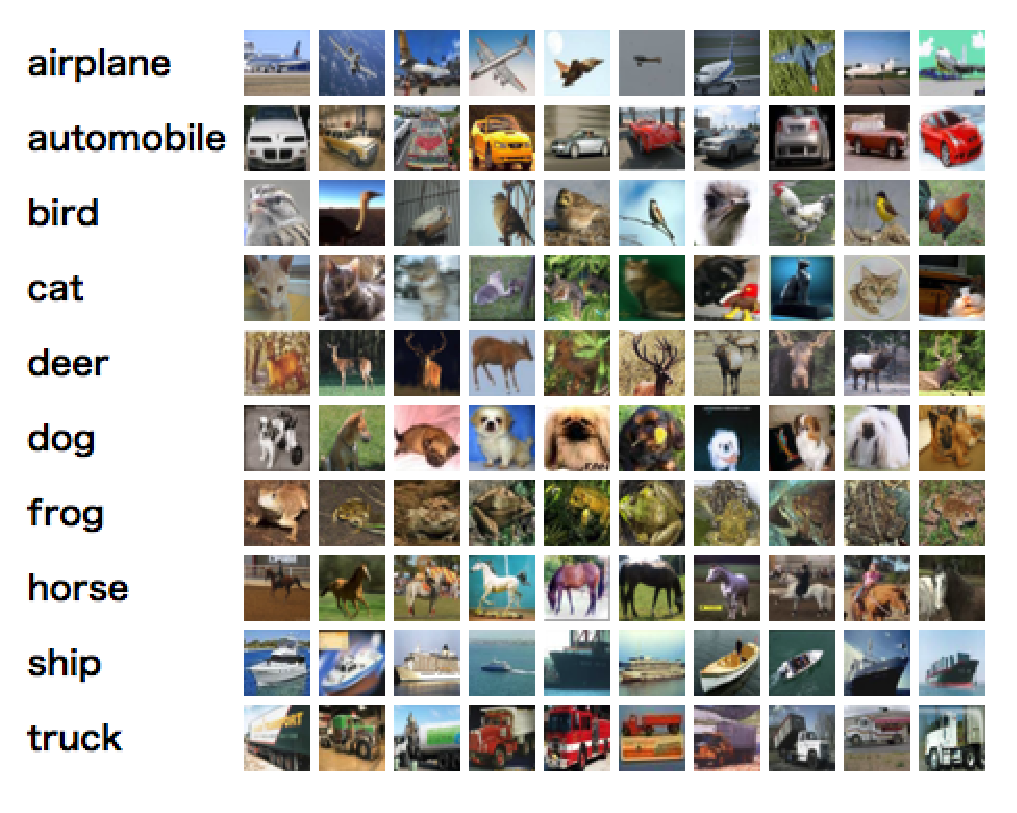
\includegraphics[width=0.8\linewidth] {images/YamasakiLab/sec2/cifar10.eps}
		\caption{CIFAR-10データセット}
		\label{fig:cifar-10}
	\end{center}
\end{figure}
\begin{practice}
dataset.pyを埋めることで,cifar10の画像を読み込むコードを完成させよ.CIFAR-10の画像はmini\_cifar/train/にある.
\end{practice}

dataset.pyを正しく書くことで以下のコマンドでCIFAR-10が実行できるようになる.
\begin{lstlisting}[basicstyle=\ttfamily\footnotesize, frame=single]
python train_cifar10_cnn.py -g 0
\end{lstlisting}
このプログラムは,mnistのプログラムとは異なり,1epochごとにmodelが出力させる.
\begin{practice}
出力されたmodelから最も精度が良いモデルを選び,そのmodelを用いて,test\_cifar10\_cnn.pyを実行せよ.
以下のコマンドでtest\_cifar10\_cnn.pyを実行できる.
\begin{lstlisting}[basicstyle=\ttfamily\footnotesize, frame=single]
python test_cifar10_cnn.py -g 0 -m (path to your model)
\end{lstlisting}
\end{practice}

\begin{practice}
(発展課題)本ネットワークの精度は約$30\sim 40$パーセントとあまり良くない.精度を上げてみよ.例えば,ネットワーク構造や,最適化手法などを変化させて見ると良い.
\end{practice}
